\subsubsection{Ý tưởng}

Shaker Sort là một biến thể của Bubble Sort, nơi mà mảng được duyệt từ trái sang phải và từ phải sang trái xen kẽ. Thuật toán này giúp giảm số lần so sánh giữa các phần tử trong mảng bằng cách sắp xếp các phần tử lớn nhất và nhỏ nhất về hai phía của mảng. \cite{black2009}

\subsubsection{Mã giả}

\begin{algorithm}[H]
\caption{Shaker Sort}
\begin{algorithmic}[1]
\Function{ShakerSort}{$arr, n$}
    \State $left \gets 0$
    \State $right \gets n - 1$
    \While{$left < right$}
        \For{$i \gets left$ \textbf{to} $right - 1$}
            \If{$arr[i] > arr[i + 1]$}
                \State \Call{Swap}{$arr[i], arr[i + 1]$}
            \EndIf
        \EndFor
        \State $right \gets right - 1$
        \For{$i \gets right$ \textbf{downto} $left + 1$}
            \If{$arr[i] < arr[i - 1]$}
                \State \Call{Swap}{$arr[i], arr[i - 1]$}
            \EndIf
        \EndFor
        \State $left \gets left + 1$
    \EndWhile
    \State \textbf{return} $arr$
\EndFunction
\end{algorithmic}
\end{algorithm}

\subsubsection{Ví dụ}
\begin{figure}[H]
    \centering
    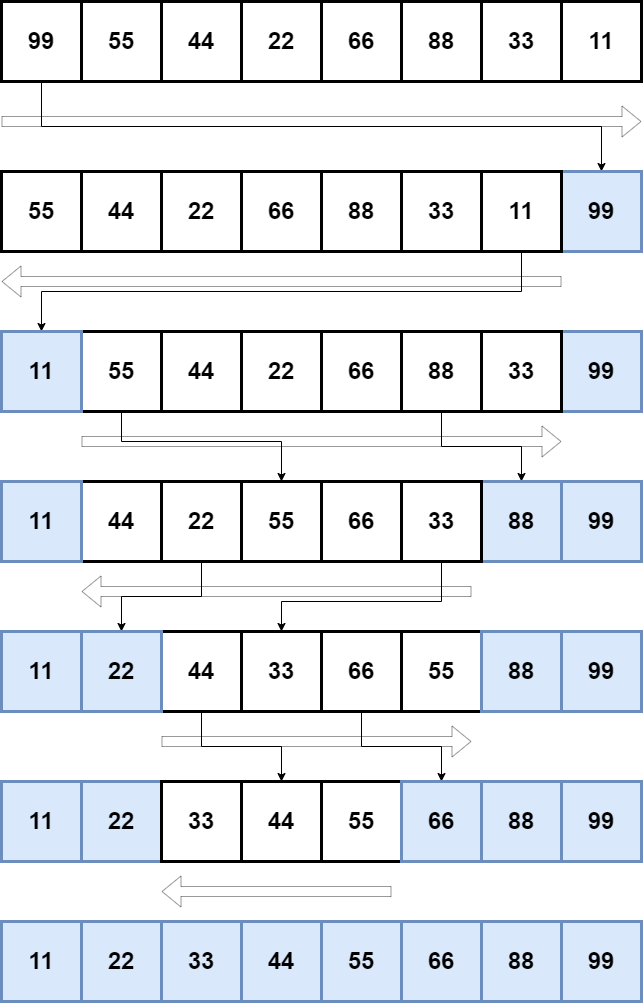
\includegraphics[width=0.6\linewidth]{img/shaker_sort/1.png}
    \caption{Quá trình thực hiện Shaker Sort}
\end{figure}

\subsubsection{Độ phức tạp}

\begin{itemize}
    \item Độ phức tạp thời gian: $O(n^2)$
    \item Độ phức tạp không gian: $O(1)$
    \item Ưu điểm:
        \begin{itemize}
            \item Giảm số lần so sánh giữa các phần tử trong mảng
        \end{itemize}
    \item Nhược điểm:
        \begin{itemize}
            \item Độ phức tạp thời gian cao
        \end{itemize}
    \item Tính ổn định: \textit{Shaker Sort} là một thuật toán ổn định. Điều này có nghĩa là nếu có hai phần tử bằng nhau, thì chúng sẽ không bị đảo lộn thứ tự sau khi sắp xếp.
    \item Ứng dụng:
        \begin{itemize}
            \item Sắp xếp các mảng có kích thước nhỏ
        \end{itemize}
\end{itemize}
